\documentclass[a4paper, 12pt]{article}
\usepackage{pgfplots, mathtools}

%% Listings With Code-Styling and Grey Background
\usepackage{float, listings} 
\lstset{						% Global Listing settings
	language=Verilog,
	numbers=left,
	numberstyle=\tiny\color{gray},
%	firstnumber=1,
	numberfirstline=true,
	stepnumber=1,
	tabsize=2,
	breaklines=true,
}
\usepackage{xcolor, mdframed, graphicx}
\definecolor{code-gray}{gray}{0.93}

%% Make specific pages landscale for larger figures
\usepackage{pdflscape}

%% Custom FSM's
\usepackage{tikz}
\usetikzlibrary{automata, positioning, arrows}
\tikzset{very thick, ->, >=stealth', node distance=6cm, every state/.style={thick, fill=gray!10}, initial text=$ $}

%% Automatic Word Formatting
\usepackage{xspace}
\newcommand*{\Vivado}{\textit{Vivado}\xspace} % Italicize Vivado
\newcommand*{\SV}{\textbf{SystemVerilog}\xspace} % Bold SystemVerilog

%% Clickable links in the output PDF
\usepackage{hyperref}
\hypersetup{colorlinks=true, linktoc=all, linkcolor=black}

%% Figure Numbering Within Sections
\let\counterwithout\relax
\let\counterwithin\relax
\usepackage{chngcntr}
\counterwithin{figure}{section}

%% Macros for logic timing diagrams
\newcounter{wavenum}
\setlength{\unitlength}{1cm}
% advance clock one cycle, not to be called directly
\newcommand*{\clki}{
  \draw (t_cur) -- ++(0,.3) -- ++(.5,0) -- ++(0,-.6) -- ++(.5,0) -- ++(0,.3)
    node[time] (t_cur) {};
}
\newcommand*{\bitvector}[3]{
  \draw[fill=#3] (t_cur) -- ++( .1, .3) -- ++(#2-.2,0) -- ++(.1, -.3)
                         -- ++(-.1,-.3) -- ++(.2-#2,0) -- cycle;
  \path (t_cur) -- node[anchor=mid] {#1} ++(#2,0) node[time] (t_cur) {};
}
% \known{val}{length}
\newcommand*{\known}[2]{
    \bitvector{#1}{#2}{white}
}
% \unknown{length}
\newcommand*{\unknown}[2][XXX]{
    \bitvector{#1}{#2}{black!20}
}
% \bit{1 or 0}{length}
\newcommand*{\bit}[2]{
  \draw (t_cur) -- ++(0,.6*#1-.3) -- ++(#2,0) -- ++(0,.3-.6*#1)
    node[time] (t_cur) {};
}
% \unknownbit{length}
\newcommand*{\unknownbit}[1]{
  \draw[ultra thick,black!50] (t_cur) -- ++(#1,0) node[time] (t_cur) {};
}
% \nextwave{name}
\newcommand{\nextwave}[1]{
  \path (0,\value{wavenum}) node[left] {#1} node[time] (t_cur) {};
  \addtocounter{wavenum}{-1}
}
% \clk{name}{period}
\newcommand{\clk}[2]{
    \nextwave{#1}
    \FPeval{\res}{(\wavewidth+1)/#2}
    \FPeval{\reshalf}{#2/2}
    \foreach \t in {1,2,...,\res}{
        \bit{\reshalf}{1}
        \bit{\reshalf}{0}
    }
}

% \begin{wave}[clkname]{num_waves}{clock_cycles}
\newenvironment{wave}[3][clk]{
  \begin{tikzpicture}[draw=black, yscale=.7,xscale=1]
    \tikzstyle{time}=[coordinate]
    \setlength{\unitlength}{1cm}
    \def\wavewidth{#3}
    \setcounter{wavenum}{0}
    \nextwave{#1}
    \foreach \t in {0,1,...,\wavewidth}{
      \draw[dotted] (t_cur) +(0,.5) node[above] {t=\t} -- ++(0,.4-#2);
      \clki
    }
}{\end{tikzpicture}}

%$ Specific Line Breaks
% See https://tex.stackexchange.com/questions/26174/ for details
\usepackage[british]{babel} 

%% Page Margins
\usepackage[margin=1.00in]{geometry}

%% Beginning of Document
\begin{document}
\counterwithin{lstlisting}{section} % Listings are numbered within sections
% Title
\title{ECE 440 - Project \#11 Simulations}
\author{Collin Heist}
\date{\today}
\maketitle

\pagenumbering{arabic}


\section{Simulations}
The AXI-traffic generator loaded all values from its data coefficient file into the FIFO sequentially, so the total post-synthesis timing simulation was quite long -- but I've included figures of the result for each factorial computation. This output is from the `perspective` of the top-level module, so it remains 0 almost always (during computation), and because of how my \textbf{XFACE} module was designed the result is cleared one clock cycle after it's found (except for the last result). This general behavior is shown clearly in the Behavioral simulation (which is identical in nature to the post-synthesis ones) shown in \textbf{Figure~\ref{fig:behav-sim}} -- however the spacing of events is more evident this way.

\begin{landscape}
\begin{figure}[H]
\centering
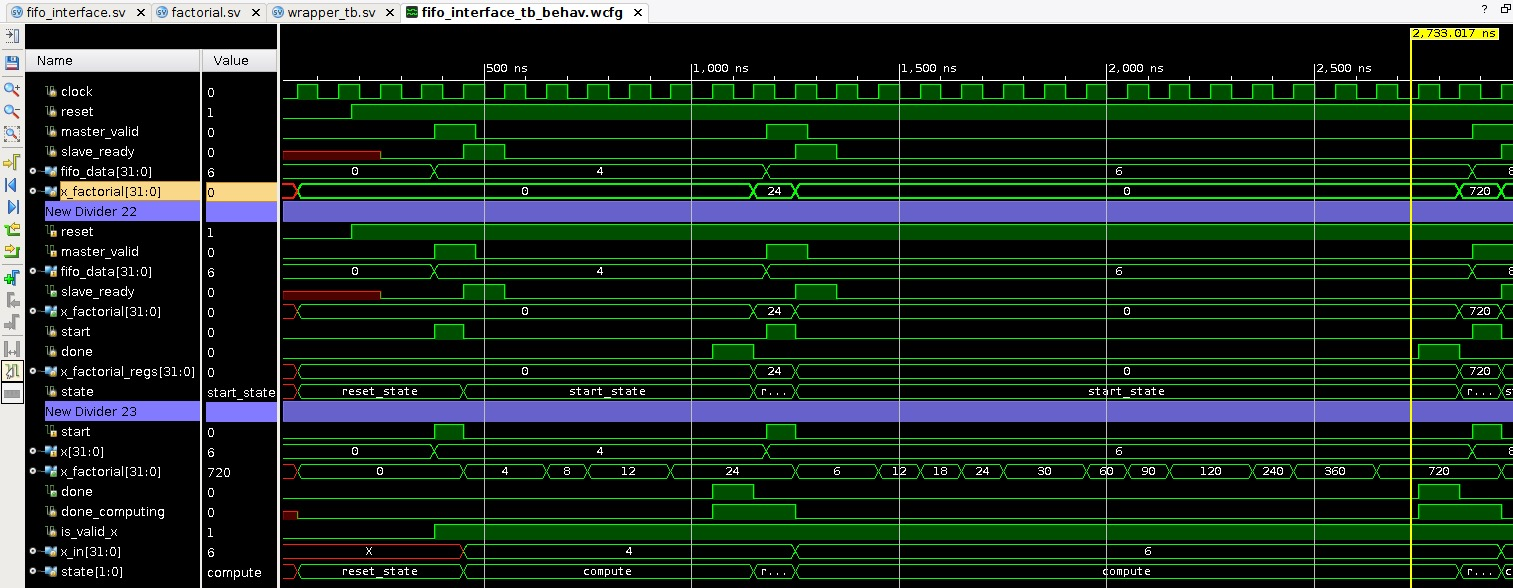
\includegraphics[width=0.80\paperheight, keepaspectratio=true]{Sources/fifo-interface-behav.jpg}
\caption{Larger behavioral simulation of the entire project -- this view clearly shows that \textbf{done} and \textbf{x\_factorial} only stay asserted for one clock cycle before moving onto the next computation.}
\label{fig:behav-sim}
\end{figure}

\begin{figure}[H]
\centering
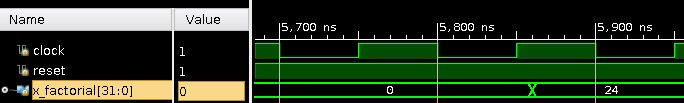
\includegraphics[width=0.80\paperheight, keepaspectratio=true]{Sources/post-impl-4.jpg}
\caption{Post-synthesis simulation of the result for $4!=24$.}
\end{figure}

\begin{figure}[H]
\centering
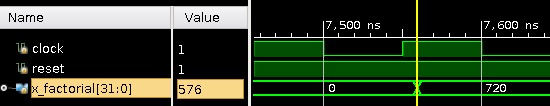
\includegraphics[width=0.80\paperheight, keepaspectratio=true]{Sources/post-impl-6.jpg}
\caption{Post-synthesis simulation of the result for $6!=720$. \textit{Note: I accidentally placed my cursor on the transition of the FFs and thus the left-value is not the final, stable value.}}
\end{figure}

\begin{figure}[H]
\centering
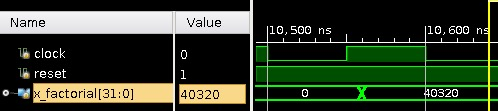
\includegraphics[width=0.80\paperheight, keepaspectratio=true]{Sources/post-impl-8.jpg}
\caption{Post-synthesis simulation of the result for $8!=420,320$.}
\end{figure}

\begin{figure}[H]
\centering
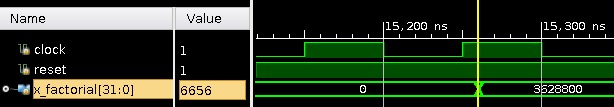
\includegraphics[width=0.80\paperheight, keepaspectratio=true]{Sources/post-impl-10.jpg}
\caption{Post-synthesis simulation of the result for $10!=3,628,800$. \textit{Note: I accidentally placed my cursor on the transition of the FFs and thus the left-value is not the final, stable value.}}
\end{figure}


\begin{figure}[H]
\centering
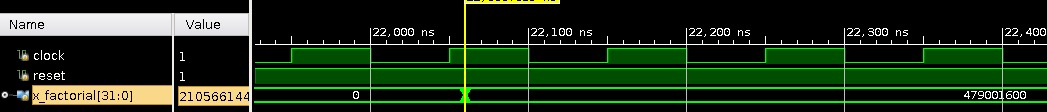
\includegraphics[width=0.80\paperheight, keepaspectratio=true]{Sources/post-impl-12.jpg}
\caption{Post-synthesis simulation of the result for $12!=479,001,600$. \textit{Note: I accidentally placed my cursor on the transition of the FFs and thus the left-value is not the final, stable value.}}
\end{figure}

\end{landscape}
\end{document}